\documentclass[12pt]{article}

%packages
%\usepackage{latexsym}
\usepackage{graphicx}
\usepackage{color}
\usepackage{amsmath}
\usepackage{dsfont}
\usepackage{placeins}
\usepackage{amssymb}
\usepackage{wasysym}
\usepackage{abstract}
\usepackage{hyperref}
\usepackage{etoolbox}
\usepackage{datetime}
\usepackage{xcolor}
\usepackage{alphalph}
\settimeformat{ampmtime}

%\usepackage{pstricks,pst-node,pst-tree}

%\usepackage{algpseudocode}
%\usepackage{amsthm}
%\usepackage{hyperref}
%\usepackage{mathrsfs}
%\usepackage{amsfonts}
%\usepackage{bbding}
%\usepackage{listings}
%\usepackage{appendix}
\usepackage[margin=1in]{geometry}
%\geometry{papersize={8.5in,11in},total={6.5in,9in}}
%\usepackage{cancel}
%\usepackage{algorithmic, algorithm}

\makeatletter
\def\maxwidth{ %
  \ifdim\Gin@nat@width>\linewidth
    \linewidth
  \else
    \Gin@nat@width
  \fi
}
\makeatother

\definecolor{fgcolor}{rgb}{0.345, 0.345, 0.345}
\newcommand{\hlnum}[1]{\textcolor[rgb]{0.686,0.059,0.569}{#1}}%
\newcommand{\hlstr}[1]{\textcolor[rgb]{0.192,0.494,0.8}{#1}}%
\newcommand{\hlcom}[1]{\textcolor[rgb]{0.678,0.584,0.686}{\textit{#1}}}%
\newcommand{\hlopt}[1]{\textcolor[rgb]{0,0,0}{#1}}%
\newcommand{\hlstd}[1]{\textcolor[rgb]{0.345,0.345,0.345}{#1}}%
\newcommand{\hlkwa}[1]{\textcolor[rgb]{0.161,0.373,0.58}{\textbf{#1}}}%
\newcommand{\hlkwb}[1]{\textcolor[rgb]{0.69,0.353,0.396}{#1}}%
\newcommand{\hlkwc}[1]{\textcolor[rgb]{0.333,0.667,0.333}{#1}}%
\newcommand{\hlkwd}[1]{\textcolor[rgb]{0.737,0.353,0.396}{\textbf{#1}}}%

\usepackage{framed}
\makeatletter
\newenvironment{kframe}{%
 \def\at@end@of@kframe{}%
 \ifinner\ifhmode%
  \def\at@end@of@kframe{\end{minipage}}%
  \begin{minipage}{\columnwidth}%
 \fi\fi%
 \def\FrameCommand##1{\hskip\@totalleftmargin \hskip-\fboxsep
 \colorbox{shadecolor}{##1}\hskip-\fboxsep
     % There is no \\@totalrightmargin, so:
     \hskip-\linewidth \hskip-\@totalleftmargin \hskip\columnwidth}%
 \MakeFramed {\advance\hsize-\width
   \@totalleftmargin\z@ \linewidth\hsize
   \@setminipage}}%
 {\par\unskip\endMakeFramed%
 \at@end@of@kframe}
\makeatother

\definecolor{shadecolor}{rgb}{.77, .77, .77}
\definecolor{messagecolor}{rgb}{0, 0, 0}
\definecolor{warningcolor}{rgb}{1, 0, 1}
\definecolor{errorcolor}{rgb}{1, 0, 0}
\newenvironment{knitrout}{}{} % an empty environment to be redefined in TeX

\usepackage{alltt}
\usepackage[T1]{fontenc}

\newcommand{\qu}[1]{``#1''}
\newcounter{probnum}
\setcounter{probnum}{1}

%create definition to allow local margin changes
\def\changemargin#1#2{\list{}{\rightmargin#2\leftmargin#1}\item[]}
\let\endchangemargin=\endlist 

%allow equations to span multiple pages
\allowdisplaybreaks

%define colors and color typesetting conveniences
\definecolor{gray}{rgb}{0.5,0.5,0.5}
\definecolor{black}{rgb}{0,0,0}
\definecolor{white}{rgb}{1,1,1}
\definecolor{blue}{rgb}{0.5,0.5,1}
\newcommand{\inblue}[1]{\color{blue}#1 \color{black}}
\definecolor{green}{rgb}{0.133,0.545,0.133}
\newcommand{\ingreen}[1]{\color{green}#1 \color{black}}
\definecolor{yellow}{rgb}{1,1,0}
\newcommand{\inyellow}[1]{\color{yellow}#1 \color{black}}
\definecolor{orange}{rgb}{0.9,0.649,0}
\newcommand{\inorange}[1]{\color{orange}#1 \color{black}}
\definecolor{red}{rgb}{1,0.133,0.133}
\newcommand{\inred}[1]{\color{red}#1 \color{black}}
\definecolor{purple}{rgb}{0.58,0,0.827}
\newcommand{\inpurple}[1]{\color{purple}#1 \color{black}}
\definecolor{backgcode}{rgb}{0.97,0.97,0.8}
\definecolor{Brown}{cmyk}{0,0.81,1,0.60}
\definecolor{OliveGreen}{cmyk}{0.64,0,0.95,0.40}
\definecolor{CadetBlue}{cmyk}{0.62,0.57,0.23,0}

%define new math operators
\DeclareMathOperator*{\argmax}{arg\,max~}
\DeclareMathOperator*{\argmin}{arg\,min~}
\DeclareMathOperator*{\argsup}{arg\,sup~}
\DeclareMathOperator*{\arginf}{arg\,inf~}
\DeclareMathOperator*{\convolution}{\text{\Huge{$\ast$}}}
\newcommand{\infconv}[2]{\convolution^\infty_{#1 = 1} #2}
%true functions

%%%% GENERAL SHORTCUTS

%shortcuts for pure typesetting conveniences
\newcommand{\bv}[1]{\boldsymbol{#1}}

%shortcuts for compound constants
\newcommand{\BetaDistrConst}{\dfrac{\Gamma(\alpha + \beta)}{\Gamma(\alpha)\Gamma(\beta)}}
\newcommand{\NormDistrConst}{\dfrac{1}{\sqrt{2\pi\sigma^2}}}

%shortcuts for conventional symbols
\newcommand{\tsq}{\tau^2}
\newcommand{\tsqh}{\hat{\tau}^2}
\newcommand{\sigsq}{\sigma^2}
\newcommand{\sigsqsq}{\parens{\sigma^2}^2}
\newcommand{\sigsqovern}{\dfrac{\sigsq}{n}}
\newcommand{\tausq}{\tau^2}
\newcommand{\tausqalpha}{\tau^2_\alpha}
\newcommand{\tausqbeta}{\tau^2_\beta}
\newcommand{\tausqsigma}{\tau^2_\sigma}
\newcommand{\betasq}{\beta^2}
\newcommand{\sigsqvec}{\bv{\sigma}^2}
\newcommand{\sigsqhat}{\hat{\sigma}^2}
\newcommand{\sigsqhatmlebayes}{\sigsqhat_{\text{Bayes, MLE}}}
\newcommand{\sigsqhatmle}[1]{\sigsqhat_{#1, \text{MLE}}}
\newcommand{\bSigma}{\bv{\Sigma}}
\newcommand{\bSigmainv}{\bSigma^{-1}}
\newcommand{\thetavec}{\bv{\theta}}
\newcommand{\thetahat}{\hat{\theta}}
\newcommand{\thetahatmle}{\hat{\theta}_{\mathrm{MLE}}}
\newcommand{\thetavechatmle}{\hat{\thetavec}_{\mathrm{MLE}}}
\newcommand{\muhat}{\hat{\mu}}
\newcommand{\musq}{\mu^2}
\newcommand{\muvec}{\bv{\mu}}
\newcommand{\muhatmle}{\muhat_{\text{MLE}}}
\newcommand{\lambdahat}{\hat{\lambda}}
\newcommand{\lambdahatmle}{\lambdahat_{\text{MLE}}}
\newcommand{\etavec}{\bv{\eta}}
\newcommand{\alphavec}{\bv{\alpha}}
\newcommand{\minimaxdec}{\delta^*_{\mathrm{mm}}}
\newcommand{\ybar}{\bar{y}}
\newcommand{\xbar}{\bar{x}}
\newcommand{\Xbar}{\bar{X}}
\newcommand{\phat}{\hat{p}}
\newcommand{\Phat}{\hat{P}}
\newcommand{\Zbar}{\bar{Z}}
\newcommand{\iid}{~{\buildrel iid \over \sim}~}
\newcommand{\inddist}{~{\buildrel ind \over \sim}~}
\newcommand{\approxdist}{~{\buildrel approx \over \sim}~}
\newcommand{\equalsindist}{~{\buildrel d \over =}~}
\newcommand{\loglik}[1]{\ell\parens{#1}}
\newcommand{\thetahatkminone}{\thetahat^{(k-1)}}
\newcommand{\thetahatkplusone}{\thetahat^{(k+1)}}
\newcommand{\thetahatk}{\thetahat^{(k)}}
\newcommand{\half}{\frac{1}{2}}
\newcommand{\third}{\frac{1}{3}}
\newcommand{\twothirds}{\frac{2}{3}}
\newcommand{\fourth}{\frac{1}{4}}
\newcommand{\fifth}{\frac{1}{5}}
\newcommand{\sixth}{\frac{1}{6}}

%shortcuts for vector and matrix notation
\newcommand{\A}{\bv{A}}
\newcommand{\At}{\A^T}
\newcommand{\Ainv}{\inverse{\A}}
\newcommand{\B}{\bv{B}}
\newcommand{\K}{\bv{K}}
\newcommand{\Kt}{\K^T}
\newcommand{\Kinv}{\inverse{K}}
\newcommand{\Kinvt}{(\Kinv)^T}
\newcommand{\M}{\bv{M}}
\newcommand{\Bt}{\B^T}
\newcommand{\Q}{\bv{Q}}
\newcommand{\Qt}{\Q^T}
\newcommand{\R}{\bv{R}}
\newcommand{\Rt}{\R^T}
\newcommand{\Z}{\bv{Z}}
\newcommand{\X}{\bv{X}}
\newcommand{\Xsub}{\X_{\text{(sub)}}}
\newcommand{\Xsubadj}{\X_{\text{(sub,adj)}}}
\newcommand{\I}{\bv{I}}
\newcommand{\Y}{\bv{Y}}
\newcommand{\sigsqI}{\sigsq\I}
\renewcommand{\P}{\bv{P}}
\newcommand{\Psub}{\P_{\text{(sub)}}}
\newcommand{\Pt}{\P^T}
\newcommand{\Pii}{P_{ii}}
\newcommand{\Pij}{P_{ij}}
\newcommand{\IminP}{(\I-\P)}
\newcommand{\Xt}{\bv{X}^T}
\newcommand{\XtX}{\Xt\X}
\newcommand{\XtXinv}{\parens{\Xt\X}^{-1}}
\newcommand{\XtXinvXt}{\XtXinv\Xt}
\newcommand{\XXtXinvXt}{\X\XtXinvXt}
\newcommand{\x}{\bv{x}}
\newcommand{\onevec}{\bv{1}}
\newcommand{\oneton}{1, \ldots, n}
\newcommand{\yoneton}{y_1, \ldots, y_n}
\newcommand{\yonetonorder}{y_{(1)}, \ldots, y_{(n)}}
\newcommand{\Yoneton}{Y_1, \ldots, Y_n}
\newcommand{\iinoneton}{i \in \braces{\oneton}}
\newcommand{\onetom}{1, \ldots, m}
\newcommand{\jinonetom}{j \in \braces{\onetom}}
\newcommand{\xoneton}{x_1, \ldots, x_n}
\newcommand{\Xoneton}{X_1, \ldots, X_n}
\newcommand{\xt}{\x^T}
\newcommand{\y}{\bv{y}}
\newcommand{\yt}{\y^T}
\renewcommand{\c}{\bv{c}}
\newcommand{\ct}{\c^T}
\newcommand{\tstar}{\bv{t}^*}
\renewcommand{\u}{\bv{u}}
\renewcommand{\v}{\bv{v}}
\renewcommand{\a}{\bv{a}}
\newcommand{\s}{\bv{s}}
\newcommand{\yadj}{\y_{\text{(adj)}}}
\newcommand{\xjadj}{\x_{j\text{(adj)}}}
\newcommand{\xjadjM}{\x_{j \perp M}}
\newcommand{\yhat}{\hat{\y}}
\newcommand{\yhatsub}{\yhat_{\text{(sub)}}}
\newcommand{\yhatstar}{\yhat^*}
\newcommand{\yhatstarnew}{\yhatstar_{\text{new}}}
\newcommand{\z}{\bv{z}}
\newcommand{\zt}{\z^T}
\newcommand{\bb}{\bv{b}}
\newcommand{\bbt}{\bb^T}
\newcommand{\bbeta}{\bv{\beta}}
\newcommand{\beps}{\bv{\epsilon}}
\newcommand{\bepst}{\beps^T}
\newcommand{\e}{\bv{e}}
\newcommand{\Mofy}{\M(\y)}
\newcommand{\KofAlpha}{K(\alpha)}
\newcommand{\ellset}{\mathcal{L}}
\newcommand{\oneminalph}{1-\alpha}
\newcommand{\SSE}{\text{SSE}}
\newcommand{\SSEsub}{\text{SSE}_{\text{(sub)}}}
\newcommand{\MSE}{\text{MSE}}
\newcommand{\RMSE}{\text{RMSE}}
\newcommand{\SSR}{\text{SSR}}
\newcommand{\SST}{\text{SST}}
\newcommand{\JSest}{\delta_{\text{JS}}(\x)}
\newcommand{\Bayesest}{\delta_{\text{Bayes}}(\x)}
\newcommand{\EmpBayesest}{\delta_{\text{EmpBayes}}(\x)}
\newcommand{\BLUPest}{\delta_{\text{BLUP}}}
\newcommand{\MLEest}[1]{\hat{#1}_{\text{MLE}}}

%shortcuts for Linear Algebra stuff (i.e. vectors and matrices)
\newcommand{\twovec}[2]{\bracks{\begin{array}{c} #1 \\ #2 \end{array}}}
\newcommand{\threevec}[3]{\bracks{\begin{array}{c} #1 \\ #2 \\ #3 \end{array}}}
\newcommand{\fivevec}[5]{\bracks{\begin{array}{c} #1 \\ #2 \\ #3 \\ #4 \\ #5 \end{array}}}
\newcommand{\twobytwomat}[4]{\bracks{\begin{array}{cc} #1 & #2 \\ #3 & #4 \end{array}}}
\newcommand{\threebytwomat}[6]{\bracks{\begin{array}{cc} #1 & #2 \\ #3 & #4 \\ #5 & #6 \end{array}}}

%shortcuts for conventional compound symbols
\newcommand{\thetainthetas}{\theta \in \Theta}
\newcommand{\reals}{\mathbb{R}}
\newcommand{\complexes}{\mathbb{C}}
\newcommand{\rationals}{\mathbb{Q}}
\newcommand{\integers}{\mathbb{Z}}
\newcommand{\naturals}{\mathbb{N}}
\newcommand{\forallninN}{~~\forall n \in \naturals}
\newcommand{\forallxinN}[1]{~~\forall #1 \in \reals}
\newcommand{\matrixdims}[2]{\in \reals^{\,#1 \times #2}}
\newcommand{\inRn}[1]{\in \reals^{\,#1}}
\newcommand{\mathimplies}{\quad\Rightarrow\quad}
\newcommand{\mathlogicequiv}{\quad\Leftrightarrow\quad}
\newcommand{\eqncomment}[1]{\quad \text{(#1)}}
\newcommand{\limitn}{\lim_{n \rightarrow \infty}}
\newcommand{\limitN}{\lim_{N \rightarrow \infty}}
\newcommand{\limitd}{\lim_{d \rightarrow \infty}}
\newcommand{\limitt}{\lim_{t \rightarrow \infty}}
\newcommand{\limitsupn}{\limsup_{n \rightarrow \infty}~}
\newcommand{\limitinfn}{\liminf_{n \rightarrow \infty}~}
\newcommand{\limitk}{\lim_{k \rightarrow \infty}}
\newcommand{\limsupn}{\limsup_{n \rightarrow \infty}}
\newcommand{\limsupk}{\limsup_{k \rightarrow \infty}}
\newcommand{\floor}[1]{\left\lfloor #1 \right\rfloor}
\newcommand{\ceil}[1]{\left\lceil #1 \right\rceil}

%shortcuts for environments
\newcommand{\beqn}{\vspace{-0.25cm}\begin{eqnarray*}}
\newcommand{\eeqn}{\end{eqnarray*}}
\newcommand{\bneqn}{\vspace{-0.25cm}\begin{eqnarray}}
\newcommand{\eneqn}{\end{eqnarray}}

%shortcuts for mini environments
\newcommand{\parens}[1]{\left(#1\right)}
\newcommand{\squared}[1]{\parens{#1}^2}
\newcommand{\tothepow}[2]{\parens{#1}^{#2}}
\newcommand{\prob}[1]{\mathbb{P}\parens{#1}}
\newcommand{\cprob}[2]{\prob{#1~|~#2}}
\newcommand{\littleo}[1]{o\parens{#1}}
\newcommand{\bigo}[1]{O\parens{#1}}
\newcommand{\Lp}[1]{\mathbb{L}^{#1}}
\renewcommand{\arcsin}[1]{\text{arcsin}\parens{#1}}
\newcommand{\prodonen}[2]{\bracks{\prod_{#1=1}^n #2}}
\newcommand{\mysum}[4]{\sum_{#1=#2}^{#3} #4}
\newcommand{\sumonen}[2]{\sum_{#1=1}^n #2}
\newcommand{\infsum}[2]{\sum_{#1=1}^\infty #2}
\newcommand{\infprod}[2]{\prod_{#1=1}^\infty #2}
\newcommand{\infunion}[2]{\bigcup_{#1=1}^\infty #2}
\newcommand{\infinter}[2]{\bigcap_{#1=1}^\infty #2}
\newcommand{\infintegral}[2]{\int^\infty_{-\infty} #2 ~\text{d}#1}
\newcommand{\supthetas}[1]{\sup_{\thetainthetas}\braces{#1}}
\newcommand{\bracks}[1]{\left[#1\right]}
\newcommand{\braces}[1]{\left\{#1\right\}}
\newcommand{\set}[1]{\left\{#1\right\}}
\newcommand{\abss}[1]{\left|#1\right|}
\newcommand{\norm}[1]{\left|\left|#1\right|\right|}
\newcommand{\normsq}[1]{\norm{#1}^2}
\newcommand{\inverse}[1]{\parens{#1}^{-1}}
\newcommand{\rowof}[2]{\parens{#1}_{#2\cdot}}

%shortcuts for functionals
\newcommand{\realcomp}[1]{\text{Re}\bracks{#1}}
\newcommand{\imagcomp}[1]{\text{Im}\bracks{#1}}
\newcommand{\range}[1]{\text{range}\bracks{#1}}
\newcommand{\colsp}[1]{\text{colsp}\bracks{#1}}
\newcommand{\rowsp}[1]{\text{rowsp}\bracks{#1}}
\newcommand{\tr}[1]{\text{tr}\bracks{#1}}
\newcommand{\rank}[1]{\text{rank}\bracks{#1}}
\newcommand{\proj}[2]{\text{Proj}_{#1}\bracks{#2}}
\newcommand{\projcolspX}[1]{\text{Proj}_{\colsp{\X}}\bracks{#1}}
\newcommand{\median}[1]{\text{median}\bracks{#1}}
\newcommand{\mean}[1]{\text{mean}\bracks{#1}}
\newcommand{\dime}[1]{\text{dim}\bracks{#1}}
\renewcommand{\det}[1]{\text{det}\bracks{#1}}
\newcommand{\expe}[1]{\mathbb{E}\bracks{#1}}
\newcommand{\expeabs}[1]{\expe{\abss{#1}}}
\newcommand{\expesub}[2]{\mathbb{E}_{#1}\bracks{#2}}
\newcommand{\indic}[1]{\mathds{1}_{#1}}
\newcommand{\var}[1]{\mathbb{V}\text{ar}\bracks{#1}}
\newcommand{\cov}[2]{\mathbb{C}\text{ov}\bracks{#1, #2}}
\newcommand{\corr}[2]{\text{Corr}\bracks{#1, #2}}
\newcommand{\se}[1]{\mathbb{S}\text{E}\bracks{#1}}
\newcommand{\seest}[1]{\hat{\mathbb{S}\text{E}}\bracks{#1}}
\newcommand{\bias}[1]{\text{Bias}\bracks{#1}}
\newcommand{\derivop}[2]{\dfrac{\text{d}}{\text{d} #1}\bracks{#2}}
\newcommand{\partialop}[2]{\dfrac{\partial}{\partial #1}\bracks{#2}}
\newcommand{\secpartialop}[2]{\dfrac{\partial^2}{\partial #1^2}\bracks{#2}}
\newcommand{\mixpartialop}[3]{\dfrac{\partial^2}{\partial #1 \partial #2}\bracks{#3}}

%shortcuts for functions
\renewcommand{\exp}[1]{\mathrm{exp}\parens{#1}}
\renewcommand{\cos}[1]{\text{cos}\parens{#1}}
\renewcommand{\sin}[1]{\text{sin}\parens{#1}}
\newcommand{\sign}[1]{\text{sign}\parens{#1}}
\newcommand{\are}[1]{\mathrm{ARE}\parens{#1}}
\newcommand{\natlog}[1]{\ln\parens{#1}}
\newcommand{\oneover}[1]{\frac{1}{#1}}
\newcommand{\overtwo}[1]{\frac{#1}{2}}
\newcommand{\overn}[1]{\frac{#1}{n}}
\newcommand{\oneoversqrt}[1]{\oneover{\sqrt{#1}}}
\newcommand{\sqd}[1]{\parens{#1}^2}
\newcommand{\loss}[1]{\ell\parens{\theta, #1}}
\newcommand{\losstwo}[2]{\ell\parens{#1, #2}}
\newcommand{\cf}{\phi(t)}

%English language specific shortcuts
\newcommand{\ie}{\textit{i.e.} }
\newcommand{\AKA}{\textit{AKA} }
\renewcommand{\iff}{\textit{iff}}
\newcommand{\eg}{\textit{e.g.} }
\newcommand{\st}{\textit{s.t.} }
\newcommand{\wrt}{\textit{w.r.t.} }
\newcommand{\mathst}{~~\text{\st}~~}
\newcommand{\mathand}{~~\text{and}~~}
\newcommand{\ala}{\textit{a la} }
\newcommand{\ppp}{posterior predictive p-value}
\newcommand{\dd}{dataset-to-dataset}

%shortcuts for distribution titles
\newcommand{\logistic}[2]{\mathrm{Logistic}\parens{#1,\,#2}}
\newcommand{\bernoulli}[1]{\mathrm{Bernoulli}\parens{#1}}
\newcommand{\betanot}[2]{\mathrm{Beta}\parens{#1,\,#2}}
\newcommand{\stdbetanot}{\betanot{\alpha}{\beta}}
\newcommand{\multnormnot}[3]{\mathcal{N}_{#1}\parens{#2,\,#3}}
\newcommand{\normnot}[2]{\mathcal{N}\parens{#1,\,#2}}
\newcommand{\classicnormnot}{\normnot{\mu}{\sigsq}}
\newcommand{\stdnormnot}{\normnot{0}{1}}
\newcommand{\uniformdiscrete}[1]{\mathrm{Uniform}\parens{\braces{#1}}}
\newcommand{\uniform}[2]{\mathrm{U}\parens{#1,\,#2}}
\newcommand{\stduniform}{\uniform{0}{1}}
\newcommand{\geometric}[1]{\mathrm{Geometric}\parens{#1}}
\newcommand{\hypergeometric}[3]{\mathrm{Hypergeometric}\parens{#1,\,#2,\,#3}}
\newcommand{\exponential}[1]{\mathrm{Exp}\parens{#1}}
\newcommand{\gammadist}[2]{\mathrm{Gamma}\parens{#1, #2}}
\newcommand{\poisson}[1]{\mathrm{Poisson}\parens{#1}}
\newcommand{\binomial}[2]{\mathrm{Binomial}\parens{#1,\,#2}}
\newcommand{\negbin}[2]{\mathrm{NegBin}\parens{#1,\,#2}}
\newcommand{\rayleigh}[1]{\mathrm{Rayleigh}\parens{#1}}
\newcommand{\multinomial}[2]{\mathrm{Multinomial}\parens{#1,\,#2}}
\newcommand{\gammanot}[2]{\mathrm{Gamma}\parens{#1,\,#2}}
\newcommand{\cauchynot}[2]{\text{Cauchy}\parens{#1,\,#2}}
\newcommand{\invchisqnot}[1]{\text{Inv}\chisq{#1}}
\newcommand{\invscaledchisqnot}[2]{\text{ScaledInv}\ncchisq{#1}{#2}}
\newcommand{\invgammanot}[2]{\text{InvGamma}\parens{#1,\,#2}}
\newcommand{\chisq}[1]{\chi^2_{#1}}
\newcommand{\ncchisq}[2]{\chi^2_{#1}\parens{#2}}
\newcommand{\ncF}[3]{F_{#1,#2}\parens{#3}}

%shortcuts for PDF's of common distributions
\newcommand{\logisticpdf}[3]{\oneover{#3}\dfrac{\exp{-\dfrac{#1 - #2}{#3}}}{\parens{1+\exp{-\dfrac{#1 - #2}{#3}}}^2}}
\newcommand{\betapdf}[3]{\dfrac{\Gamma(#2 + #3)}{\Gamma(#2)\Gamma(#3)}#1^{#2-1} (1-#1)^{#3-1}}
\newcommand{\normpdf}[3]{\frac{1}{\sqrt{2\pi#3}}\exp{-\frac{1}{2#3}(#1 - #2)^2}}
\newcommand{\normpdfvarone}[2]{\dfrac{1}{\sqrt{2\pi}}e^{-\half(#1 - #2)^2}}
\newcommand{\chisqpdf}[2]{\dfrac{1}{2^{#2/2}\Gamma(#2/2)}\; {#1}^{#2/2-1} e^{-#1/2}}
\newcommand{\invchisqpdf}[2]{\dfrac{2^{-\overtwo{#1}}}{\Gamma(#2/2)}\,{#1}^{-\overtwo{#2}-1}  e^{-\oneover{2 #1}}}
\newcommand{\exponentialpdf}[2]{#2\exp{-#2#1}}
\newcommand{\poissonpdf}[2]{\dfrac{e^{-#1} #1^{#2}}{#2!}}
\newcommand{\binomialpdf}[3]{\binom{#2}{#1}#3^{#1}(1-#3)^{#2-#1}}
\newcommand{\rayleighpdf}[2]{\dfrac{#1}{#2^2}\exp{-\dfrac{#1^2}{2 #2^2}}}
\newcommand{\gammapdf}[3]{\dfrac{#3^#2}{\Gamma\parens{#2}}#1^{#2-1}\exp{-#3 #1}}
\newcommand{\cauchypdf}[3]{\oneover{\pi} \dfrac{#3}{\parens{#1-#2}^2 + #3^2}}
\newcommand{\Gammaf}[1]{\Gamma\parens{#1}}

%shortcuts for miscellaneous typesetting conveniences
\newcommand{\notesref}[1]{\marginpar{\color{gray}\tt #1\color{black}}}

%%%% DOMAIN-SPECIFIC SHORTCUTS

%Real analysis related shortcuts
\newcommand{\zeroonecl}{\bracks{0,1}}
\newcommand{\forallepsgrzero}{\forall \epsilon > 0~~}
\newcommand{\lessthaneps}{< \epsilon}
\newcommand{\fraccomp}[1]{\text{frac}\bracks{#1}}

%Bayesian related shortcuts
\newcommand{\yrep}{y^{\text{rep}}}
\newcommand{\yrepisq}{(\yrep_i)^2}
\newcommand{\yrepvec}{\bv{y}^{\text{rep}}}


%Probability shortcuts
\newcommand{\SigField}{\mathcal{F}}
\newcommand{\ProbMap}{\mathcal{P}}
\newcommand{\probtrinity}{\parens{\Omega, \SigField, \ProbMap}}
\newcommand{\convp}{~{\buildrel p \over \rightarrow}~}
\newcommand{\convLp}[1]{~{\buildrel \Lp{#1} \over \rightarrow}~}
\newcommand{\nconvp}{~{\buildrel p \over \nrightarrow}~}
\newcommand{\convae}{~{\buildrel a.e. \over \longrightarrow}~}
\newcommand{\convau}{~{\buildrel a.u. \over \longrightarrow}~}
\newcommand{\nconvau}{~{\buildrel a.u. \over \nrightarrow}~}
\newcommand{\nconvae}{~{\buildrel a.e. \over \nrightarrow}~}
\newcommand{\convd}{~{\buildrel \mathcal{D} \over \rightarrow}~}
\newcommand{\nconvd}{~{\buildrel \mathcal{D} \over \nrightarrow}~}
\newcommand{\withprob}{~~\text{w.p.}~~}
\newcommand{\io}{~~\text{i.o.}}

\newcommand{\Acl}{\bar{A}}
\newcommand{\ENcl}{\bar{E}_N}
\newcommand{\diam}[1]{\text{diam}\parens{#1}}

\newcommand{\taua}{\tau_a}

\newcommand{\myint}[4]{\int_{#2}^{#3} #4 \,\text{d}#1}
\newcommand{\laplacet}[1]{\mathscr{L}\bracks{#1}}
\newcommand{\laplaceinvt}[1]{\mathscr{L}^{-1}\bracks{#1}}
\renewcommand{\min}[1]{\text{min}\braces{#1}}
\renewcommand{\max}[1]{\text{max}\braces{#1}}

\newcommand{\Vbar}[1]{\bar{V}\parens{#1}}
\newcommand{\expnegrtau}{\exp{-r\tau}}

%%% problem typesetting
\definecolor{darkgrey}{rgb}{0.10,0.10,0.9}

\newcommand{\problem}[1]{\noindent \colorbox{black}{{\color{yellow} \large{\textsf{\textbf{Problem \arabic{probnum}}}}~}} \addtocounter{probnum}{1} \vspace{0.2cm} \\ \iftoggle{professormode}{}{\color{darkgrey}} #1}

\newcommand{\easysubproblem}[1]{\ingreen{\item} \iftoggle{professormode}{}{\color{darkgrey}} [easy] #1 \color{black} }
\newcommand{\intermediatesubproblem}[1]{\inorange{\item} \iftoggle{professormode}{}{\color{darkgrey}} [harder] #1 \color{black} }
\newcommand{\hardsubproblem}[1]{\inred{\item} \iftoggle{professormode}{}{\color{darkgrey}} [difficult] #1 \color{black} }
\newcommand{\extracreditsubproblem}[1]{\inpurple{\item} \iftoggle{professormode}{}{\color{darkgrey}} [E.C.] #1 \color{black} }


\newcommand{\spc}[1]{\iftoggle{professormode}{\\ \vspace{#1cm}}{\\ \vspace{-0.3cm}}}

\makeatletter
\newalphalph{\alphmult}[mult]{\@alph}{26}
\renewcommand{\labelenumi}{(\alphmult{\value{enumi}})}

\newcommand{\support}[1]{\text{Supp}\bracks{#1}}
\newcommand{\mode}[1]{\text{Mode}\bracks{#1}}
\newcommand{\IQR}[1]{\text{IQR}\bracks{#1}}
\newcommand{\quantile}[2]{\text{Quantile}\bracks{#1,\,#2}}
\usepackage{xcolor}
\usepackage{graphicx}


\newtoggle{professormode}
% \toggletrue{professormode} %STUDENTS: DELETE or COMMENT this line



\title{MATH 342W / 650.4 Spring \the\year ~Homework \#3}

\author{Loyd Flores} %STUDENTS: write your name here

\iftoggle{professormode}{
\date{Due 11:59PM March 17 \\ \vspace{0.5cm} \small (this document last updated \currenttime~on \today)}
}

\renewcommand{\abstractname}{Instructions and Philosophy}

\begin{document}
\maketitle

\iftoggle{professormode}{
\begin{abstract}
The path to success in this class is to do many problems. Unlike other courses, exclusively doing reading(s) will not help. Coming to lecture is akin to watching workout videos; thinking about and solving problems on your own is the actual ``working out.''  Feel free to \qu{work out} with others; \textbf{I want you to work on this in groups.}

Reading is still \textit{required}. You should be googling and reading about all the concepts introduced in class online. This is your responsibility to supplement in-class with your own readings.

The problems below are color coded: \ingreen{green} problems are considered \textit{easy} and marked \qu{[easy]}; \inorange{yellow} problems are considered \textit{intermediate} and marked \qu{[harder]}, \inred{red} problems are considered \textit{difficult} and marked \qu{[difficult]} and \inpurple{purple} problems are extra credit. The \textit{easy} problems are intended to be ``giveaways'' if you went to class. Do as much as you can of the others; I expect you to at least attempt the \textit{difficult} problems. 

This homework is worth 100 points but the point distribution will not be determined until after the due date. See syllabus for the policy on late homework.

Up to 7 points are given as a bonus if the homework is typed using \LaTeX. Links to instaling \LaTeX~and program for compiling \LaTeX~is found on the syllabus. You are encouraged to use \url{overleaf.com}. If you are handing in homework this way, read the comments in the code; there are two lines to comment out and you should replace my name with yours and write your section. The easiest way to use overleaf is to copy the raw text from hwxx.tex and preamble.tex into two new overleaf tex files with the same name. If you are asked to make drawings, you can take a picture of your handwritten drawing and insert them as figures or leave space using the \qu{$\backslash$vspace} command and draw them in after printing or attach them stapled.

The document is available with spaces for you to write your answers. If not using \LaTeX, print this document and write in your answers. I do not accept homeworks which are \textit{not} on this printout. Keep this first page printed for your records.

\end{abstract}

\thispagestyle{empty}
\vspace{1cm}
NAME: \line(1,0){380}
\clearpage
}

\problem{These are questions about Silver's book, chapters 3-6.  For all parts in this question, answer using notation from class (i.e. $t ,f, g, h^*, \delta, \epsilon, e, t, z_1, \ldots, z_t, \mathbb{D}, \mathcal{H}, \mathcal{A}, \mathcal{X}, \mathcal{Y}, X, y, n, p, x_{\cdot 1}, \ldots, x_{\cdot p}$, $x_{1 \cdot}, \ldots, x_{n \cdot}$, etc.} % and also we now have $f_{pr}, h^*_{pr}, g_{pr}, p_{th}$, etc from probabilistic classification as well as different types of validation schemes)

\begin{enumerate}

\hardsubproblem{Chapter 4 is all about predicting weather. Broadly speaking, what is the problem with weather predictions? Make sure you use the framework and notation from class. This is not an easy question and we will discuss in class. Do your best.}\spc{6} \\
The world in itself is very complex. There are too many reasons for why things occur, too many variables to consider, we can never completely know what goes on in a phenomena, the best we can do is approximate. Weather is a different beast. It is a dynamic system where the tiniest things could drastically alter the outcome. This is one reason why predicting the weather is hard. There exists limitation on how much we  understand the world. Due to it's complexity it makes it even harder to collect the right data to input into our models. For example, even thermometers make mistakes. As stated in Silver's book, they may even be off just in the third or fourth decimal place. According to the principles of chaos theory and the nature of weather prediction as a dynamic system implies that fundamentally there is already error occurring and piling up. Our prediction from the start is immediately wrong. In the context of our lectures there exists such \( z_1, z_2, \ldots, z_n \), which are real drivers of a phenomena. We may never even grasp the \( z's \) that's why the best we can do is approximate them with \( x's \), which again makes our predictions wrong. Returning back on the idea of Weather being a dynamic system, that in itself also poses another problem. The features we use to predict today may not be of significance in the future. We may find other reasons as to why the weather changes thus debunking methodologies we used in the past. Weather is not stationary and a multitude of factors may contribute to the change of weather and temperature. Lastly, despite computing power improving exponentially in recent decades it still isn't enough. Our ability to compute the weather has long lagged behind our theoretical understanding of it. We know which equations to solve and roughly what the answers are , but we aren't fast enough to calculate tehem for every molecule in the earth's atmosphere, again because the world is too complex. \\

\easysubproblem{Why does the weatherman lie about the chance of rain? And where should you go if you want honest forecasts?}\spc{2} \\ 
According to the findings of Eric Floehr, That statistical reality of accuracy isn't the governing paradigm when it comes to commercial weather forecasting. In simpler terms commercial weather providers have less incentive to give the most accurate predictions and trade-off some accuracy to fuel their personal agendas. Most commercial weather forecasts predict more precipitation than what actually occurs. Meteorologists call this "wet bias". For example if the prediction comes out to be a 5\%, they instead inflate it to be 20\%. By doing this commercial weather forecasts gain more profit because they "add value" by subtracting accuracy. According to Floehr if you want the most accurate forecasts you must result to the source, the government's data. All the commercial providers source their data from here before aggregating their own biases onto the data. The further you are from source the less accurate it becomes.

\hardsubproblem{Chapter 5 is all about predicting earthquakes. Broadly speaking, what is the problem with earthquake predictions? It is \textit{not} the same as the problem of predicting weather. Read page 162 a few times. Make sure you use the framework and notation from class.}\spc{5} \\ 

Both weather and earthquakes are dynamic systems. There are a multitude of factors that could affect these natural phenomena from occurring and a slight mishap in calculation could render our model to occur more error. The first major difference is that meteorologists are approximating the \( z's \) more accurately. This roots from the better understanding of meteorologists on weather's phenomena or dynamic system as to seismologists to the phenomena of earthquakes. For example they have a strong fundamental understanding of what causes tornadoes and how they dissipate and seismologists are still trying to find out for sure what happens before or after an earthquake. Therefore models predicting earthquakes will incur larger \( \delta \), or error due to ignorance, there are just more things that seismologists are unaware of. A possible cause could be that weather has a richer dataset \( \mathbb{D} \) available since earthquakes happen less frequently. A lot of earthquakes occur but they all vary in strength. Weaker ones happen more frequently and some even go unnoticed or unregistered while stronger ones happen so infrequently that we can't even begin to pick up the patterns. There is an obvious difference in the availability of data and understanding of phenomena. Secondly weather has a larger array of out of sample validation techniques that it can rely on. Persistence, climatology, and larger amounts of data is available for weather meanwhile earthquakes can only be validated once they occur. In the terms of our lecture, weather has better validation techniques and is even able to split its dataset \( \mathbb{D} \)  into  \( D_{\text{test}} \) and \( D_{\text{train}} \)
, while earthquakes don't really have the same luxury. Earthquake prediction desperately seeks signal while weather is gradually developing their approximations to \( f \). \\  \\
\easysubproblem{Silver has quite a whimsical explanation of overfitting on page 163 but it is really educational! What is the nonsense predictor in the model he describes?}\spc{2} \\ 

As discussed in Page 163 most economists rely on their judgement to some degree when making a forecast rather than just taking the output of a statistical model as is. Which could be simplified using the a quote from \textit{George Box} which states: "All models are wrong but some are useful." It is then necessary that judgemental adjustments are made to the statistical model to make them better which was proven in the study of \textit{Stephen K. McNess}, adjusted models performed 15\% better because relying solely on statistical methods and computational resources will not account for the lack of theoretical understanding about a phenomena. What he was discussing as the non-sense predictor is when too much judgment is introduced it turns into bias. The amount of bias that could be incurred depends on the influence of reputation. The less known you are the less you have to lose by taking a big risk when predicting. Conversely if you have a good reputation you might be reluctant to step too far out of the line even if data demands it. Either of these concerns potentially distracts you from the goal of making the most honest predictions. The data collected from the Survey of Professional Forecasters proves that anonymous predictions always performed better because there are less biases and personal interests are added onto the model due to anonymity being lower stakes.

\easysubproblem{John von Neumann was credited with saying that \qu{with four parameters I can fit an elephant and with five I can make him wiggle his trunk}. What did he mean by that and what is the message to you, the budding data scientist? }\spc{5} \\ 

Over fitting is a big topic in this part of the text. It occurs when a model captures the noise rather than the underlying signal, resulting in a model that performs well on the training data but poorly on new, unseen data. In the context of our class an over-fit model understands the variability of the data it is fed which in the class' context means the model has an \( R^2\) which is closer to one, in the context of this text it was 85\% . Although these in-sample metrics are amazing they do not tell the entire truth. If anything they are deceiving you. The model fails to generalize new or unseen data. The quote \textbf{"With four parameters I can fit an elephant"} implies that the possibilities for an over fit model are endless even with a small feature count of 4. It emphasizes this even more by stating \textbf{"With five I can make him wiggle his trunk"} that the addition of more noise could drastically increase the complexity of our model. This implies that our model is so delusional that because it fully understood the noise and its complexity which places us further away from the actual phenomena we are interested in.  \\ \\ \\ \\

\hardsubproblem{Chapter 6 is all about predicting unemployment, an index of macroeconomic performance of a country. Broadly speaking, what is the problem with unemployment predictions? It is \textit{not} the same as the problem of predicting weather or earthquakes. Make sure you use the framework and notation from class.}\spc{6} \\ 

Predicting unemployment is different from weather or earthquakes because it has even less data available while being more complex. The nature of employment and economy is a different level of complex, there are so many indicators that you could possibly consider. It also requires a really complex model to understand the large variability in this field. In the context of the lectures the problem with unemployment predictions is that we are unable to properly identify the proper approximation \(x\) to the \(z's\). There are so many interconnected variables from small consumer behavior to large global movements of the market.  All these indicators are dynamic and we can't keep track of them which increases \( \delta \) that our model is incurring or the error due to ignorance. Economic models also require a lot more subjective judgement allowing over-fitting wreak havoc easily. With the complex nature of the economy, it is harder to approximate \(f\), increasing our misspecification error due to the limited nature of existing models. Overall the problem is just completely different in complexity. It stems from the unique and complex nature of economic systems, which pose challenges beyond those encountered in weather or earthquakes.
 

\extracreditsubproblem{Many times in this chapter Silver says something on the order of \qu{you need to have theories about how things function in order to make good predictions.} Do you agree? Discuss.}\spc{13} \\ 
I agree with this statement. To solve a problem you must first understand the problem. For example you may memorize all the mathematical formulas in this world but if you are unable to understand the problem the knowledge you posses is rendered unusable due to the fact that you are unable to apply it. The same could be said in the context of Data Science and Machine Learning. How will you solve problems if you don't know how they fundamentally occur? The lack of theory presents a worse approximation of \(x's\) to \(z's\). There is also room for oversimplifying the problem which leads to a model that also fails to approximate \(f\). For someone to produce a model that works and is useful they must first understand what they are trying to achieve, this is done by understanding the theories that govern the desired target. Secondly, theory in the domains of machine learning and data science are also necessary to be able to interpret and utilize the available data. What is a science textbook to a dogmatic and religious fundamentalist, nothing because it is virtually blasphemous garbage to them.


\end{enumerate}
\newpage


\problem{These are questions related to the concept of orthogonal projection, QR decomposition and its relationship with least squares linear modeling.} 

\begin{enumerate}

\easysubproblem{Let $\H$ be the orthogonal projection onto $\colsp{\X}$ where $\X$ is a $n \times (p+1)$ matrix with all columns linearly independent from each other. What is $\rank{\H}$?}\spc{0.5} \\

If matrix \( X\) is size \( n * (p + 1)\) then rank[\(H\)] = \(p + 1\) should also hold because the rank of \(H\) is purely determined by the number of linearly independent columns in \(X\) which is \(p + 1\). The dimension of the column space of \(X\) is dictated by \(n\), thus rank[\(H\)] = \(p + 1\)


\easysubproblem{Simplify $\H\X$ by substituting for $\H$.}\spc{0.5} \\ 
= \textcolor{red}{\(H\)}\(X\) = \(X\), this could also be written as : \\
= \textcolor{red}{\(H\)}\(X\) = \textcolor{red}{\( X(X^T X)^{-1} X^T\)} X = X\\
= \textcolor{red}{\(H\)}\(X\) = \(X * I\) = X


\intermediatesubproblem{What does your answer from the previous question mean conceptually?}\spc{2} \\ 

The previous problem indicates that the effect of the \textbf{orthogonal projection matrix} \(H\) on matrix \(X\) is equivalent to simply leaving \(X\) unchanged. It aligns with the fundamental understanding of orthogonal projection, where vectors projected onto a subspace remain unchanged if they already lie within that subspace.

\hardsubproblem{Let $\X'$ be the matrix of $\X$ whose columns are in reverse order meaning that $\X = [ \onevec_n~\vdots~\x_{\cdot 1}~\vdots~ \ldots~\vdots~ \x_{\cdot p} ]$ and $\X' = [\x_{\cdot p}~\vdots~ \ldots~\vdots~\x_{\cdot 1}~\vdots~\onevec_n]$. Show that the projection matrix that projects onto $\colsp{X}$ is the same exact projection matrix that projects onto $\colsp{X'}$.}\spc{4} \\
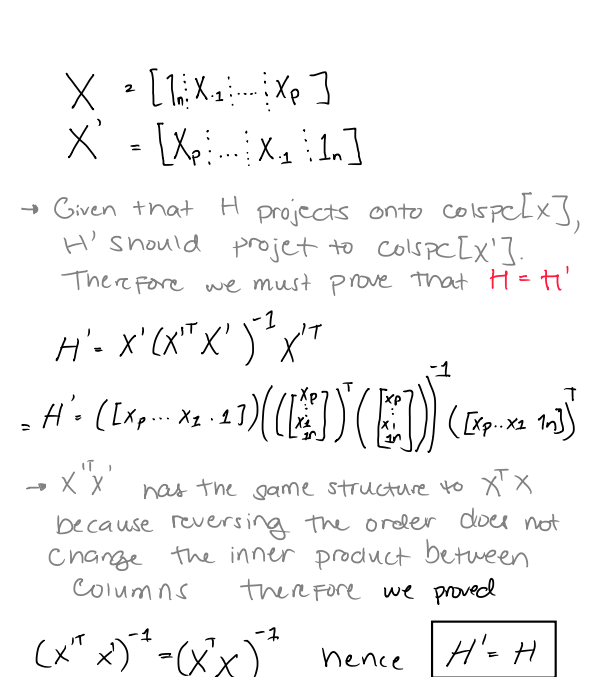
\includegraphics[width=0.4\textwidth]{2d.png}

% \hardsubproblem{[MA] Generalize the previous problem by proving that orthogonal projection matrices that project onto any specific subspace are \emph{unique}.}\spc{10}

% \hardsubproblem{[MA] Prove that if a square matrix is both symmetric and idempotent then it must be an orthogonal projection matrix.}\spc{10}

\easysubproblem{Prove that $I_n$ is an orthogonal projection matrix $\forall n$.}\spc{3} \\
For something to be an orthogonal projection matrix it must satisfy two conditions, \textbf{Symmetry} and \textbf{Impotence}. In the case of \(I_n\) by definition it is the identity matrix meaning that all diagonal elements are 1 and the rest are 0's. Since it is the identity it has to be square. Multiplying such matrix by itself you obtain yourself or \(I_n^{2}\) = \(I_n\) which satisfy the condition of \textbf{symmetry}. Another implication of \(I_n\) being square is that if transpose or swap the rows and columns it does not change the structure or \(I_n^{T}\) = \(I_n\) satisfying the second condition of \textbf{idempotency}. \\ \\ \\


\easysubproblem{What subspace does $I_n$ project onto?}\spc{3} \\
The identity matrix \(I_n\) projects onto the entire subspace of \( \mathbb{R}^{2} \) because as the identity matrix it preserves all vectors in \( \mathbb{R}^{2} \) without changing the direction or magnitude of any vector \(v\). When we apply the projection operation using \(I_n\) we get the same vector back or \(I_n\)v = v. \\

\easysubproblem{Consider least squares linear regression using a design matrix $X$ with rank $p + 1$. What are the degrees of freedom in the resulting model? What does this mean?}\spc{3} \\ 
If rank[\(X\)] = \(p+1\), its degrees of freedom would also be p+1. The Degrees of freedom just imply the number of linearly independent columns we have that can capture the variability in the response variable. In simpler terms we have more independent pieces of information to explain our target hence why "degrees of freedom capture variability."


\easysubproblem{If you are orthogonally projecting the vector $\y$ onto the column space of $X$ which is of rank $p + 1$, derive the formula for $\proj{\colsp{X}}{\y}$. Is this the same as in OLS?}\spc{8} \\ 
To project \(y\) onto the colspc[\(X\)], the projection matrix could be denoted as \(H\) = \(X (X^T X)^{-1} X^T\). Substituting that we get: \\
= \(Proj_{colsp[x]} (y)\) =  \((X (X^T X)^{-1} X^T)y \) \\ 

In OLS the goal is the find the coefficients \( \beta \) that minimize the residual sum of squares,
\( \beta \) is denoted by : \\
\( \beta\) = \((X^T X)^{-1} X^T)y \) \\

We can substitute the OLS solution by plugging in \( \beta \) : \\
\(Proj_{colsp[x]} (y)\) =  \((X (X^T X)^{-1} X^T)y \) = X\( \beta \). Therefore in the context of OLS regression, the projection of \(y\) into \(colsp[x]\) is the same as the predicted values of y from the regression model.
 
\hardsubproblem{We saw that the perceptron is an \textit{iterative algorithm}. This means that it goes through multiple iterations in order to converge to a closer and closer $\bv{w}$. Why not do the same with linear least squares regression? Consider the following. Regress $\y$ using $\X$ to get $\yhat$. This generates residuals $\e$ (the leftover piece of $\y$ that wasn't explained by the regression's fit, $\yhat$). Now try again! Regress $\e$ using $\X$ and then get new residuals $\e_{new}$. Would $\e_{new}$ be closer to $\bv{0}_n$ than the first $\e$? That is, wouldn't this yield a better model on iteration \#2? Yes/no and explain.}\spc{10} \\
The second regression on the residuals may not necessarily result in \( \hat{e}_{new}\) that is closer to \(0_n\) than the initial residual \(e\) because the initial regression already captures the variation in y explained by the predictors in \(X\). The remaining variation captured by the residuals may not be effectively modeled by the same predictors in \(X\), since we are using the same input matrix \(X\) for the succeeding iterations. Thus implying that iterative regression on the residuals may not significantly improve the modal and may not converge to a better solution compared to iterative method that perception uses that it gradually fixes the fit of the line.


\intermediatesubproblem{Prove that $\Q^\top = \Q^{-1}$ where $\Q$ is an orthonormal matrix such that $\colsp{\Q} = \colsp{\X}$ and $\Q$ and $\X$ are both matrices $\in \reals^{n \times (p+1)}$ and $n = p+1$ in this case to ensure the inverse is defined. Hint: this is purely a linear algebra exercise and it's a one-liner.}\spc{2} \\ 
Since \(Q\) is an \textbf{orthonormal  matrix} its transpose \(Q^T\) is also its inverse. This is the fundamental idea of orthonormal  matrices that they have orthogonal columns and unit length, when transposed they maintain their orthogonality and unit length thus proving
\textbf{\(Q^{-1}\) = \(Q^T\)}


\easysubproblem{Prove that the least squares projection $\H = \XXtXinvXt = \Q\Q^\top$. Justify each step.}\spc{3} \\ 
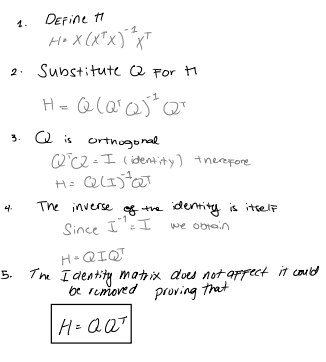
\includegraphics[width=0.5\textwidth]{2k.png} \\ \\ 


% \hardsubproblem{[MA] This problem is independent of the others. Let $H$ be an orthogonal projection matrix. Prove that $\rank{\H} =\tr{\H}$. Hint: you will need to use facts about eigenvalues and the eigendecomposition of projection matrices.}\spc{12}

\intermediatesubproblem{Prove that an orthogonal projection onto the $\colsp{\Q}$ is the same as the sum of the projections onto each column of $\Q$.}\spc{9} \\
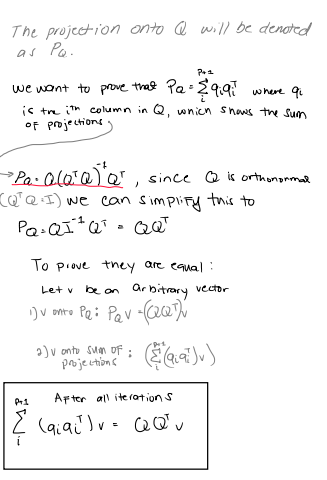
\includegraphics[width=0.4\textwidth]{2i.png}

\easysubproblem{Explain why adding a new column to $\X$ results in no change in the SST remaining the same.}\spc{1} \\ 
SST or Sum squared total is a measure of the total variability present in the dependent variable \(y\) without considering any predictors. This is crucial because it provides a baseline understanding of how much the observed values of \(y\) deviate from their mean. SST is derived from SST =  \( \sum\limits_{i=1}^n (y_i - \bar{y})^2 \) adding more X's or feature columns won't really affect the variability of y. 

\intermediatesubproblem{Prove that adding a new column to $\X$ results in SSR increasing.}\spc{4} \\
SSR or Sum squared Residual represents the sum of the squared difference between the predicted values of the dependent variable \( \hat{y}\) and the mean of the dependent variable \(\bar{y}\) or SSR = \(\sum\limits_{i=1}^n\)(\(\hat{y} - \bar{y})^2\). When we add a new column \(X_{new}\) to the predictor matrix \(X\) it means that we're introducing a new predictor or feature. When we fit a linear regression model with the new predictor included. When the model attempts to explain more of the variability in the dependent variable incorporating all the features in \(X\) including \(X_{new}\) the values of \( \hat{y}\) will probably change and will be closer to 0 therefore changing the value of SSR because the larger difference from \( \hat{y} \) - \( \bar{y}\) will result into a larger SSR when squared. \\ \\

\intermediatesubproblem{What is overfitting? Use what you learned in this problem to frame your answer.}\spc{4} \\
Overfitting occurs when our model oversimplifies a problem by fully understanding the patterns and noise found in the data it was trained on. It then fails to generalize on new and or unseen data. If I am using concepts from the previous questions, if we keep adding garbage features our model will become more complex and we will have a better fit line that includes the garbage. SSR will keep increasing which is a strong indicator of overfitting.

\easysubproblem{Why are \qu{in-sample} error metrics (e.g. $R^2$, SSE, $s_e$) dishonest? Note: I'm leaving out RMSE as RMSE attempts to be honest by increasing as $p$ increases due to the denominator. I've chosen to use standard error of the residuals as the error metric of choice going forward.}\spc{5} \\ 
In sample error metrics are dishonest because they are calculated using the same data the model was trained on. This means they can overly reward complex models that fit the noise in the data rather than the true pattern it needs. Better scores on in-simple metrics may lead you to think that you have an amazing model when in reality it won't really know how to deal with new or unseen data. 

\easysubproblem{How can we provide honest error metrics (e.g. $R^2$, SSE, $s_e$)? It may help to draw a picture of the procedure.}\spc{14} \\ 
To provide honest error metrics that accurately relfect the performance of a model, we need to verify it with data it has not seen. A model has to be validated with out-of-sample evaluation methods. One approach that we can do is split our \( \mathcal{D}\) into \( \mathcal{D}_{test} \) and \( \mathcal{D}_{train} \), where \( \mathcal{D}_{train} \) will be used to train our model and the remaining \( \mathcal{D}_{test} \) will be used to validate our model using out-of-sample data. \\
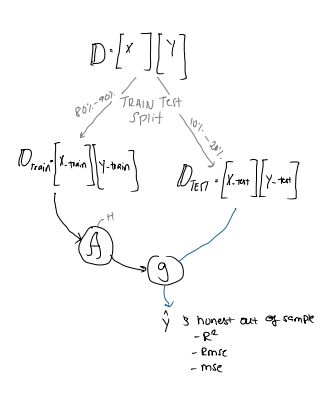
\includegraphics[width=0.4\textwidth]{3q.png} \\


\easysubproblem{The procedure in (t) produces highly variable honest error metrics. Can you change the procedure slightly to reduce the variation in the honest error metrics? What is this procedure called and how is it done?}\spc{6} \\ 
To produce more stable metrics we deploy a process called \textbf{K-fold cross validation}, which splits our data into \textbf{k} folds. For example we set \textbf{k} = 5, this splits up the data into 5 folds. We then train 5 different models on these folds. Each model will then use one fold to validate and the rest to train. For example \(model_1\) trains on \(fold_{2..n}\) and uses \(fold_{1}\) to validate. This repeats for all models and we average all the residuals to create a more stable metric.




\end{enumerate}

\newpage
\problem{These are some questions related to validation.}

\begin{enumerate}

\easysubproblem{Assume you are doing one train-test split where you build the model on the training set and validate on the test set. What does the constant $K$ control? And what is its tradeoff?}\spc{4} \\ 
\(K\) is a hyper parameter that could be selected, it signifies how you'll split the data. A low \(K\) means you'll have fewer data points in your test set, which could lead to higher bias in your evaluation because the model's performance could be sensitive to a particular subset of data for testing. A high \(K\) means you have more data points in your test set which could help reduce bias. However, this might increase variance because your averaging over more test sets leading to a wider range of performance metrics. To summarize, \(K\) controls the bias-variance trade off in models.

\intermediatesubproblem{Assume you are doing one train-test split where you build the model on the training set and validate on the test set. If $n$ was very large so that there would be trivial misspecification error even when using $K=2$, would there be any benefit at all to increasing $K$ if your objective was to estimate generalization error? Explain.}\spc{4} \\ 
If n is very large and there is trivial misspecification error present a larger n may still contain the same misspecification error accounted for. Since there is a large n our model probably fit the noise as well. The only way to develop our model is by picking a more complex set of functions in our \(H\). In the end when trivial misspecification is present there is no benefit in increasing \(K\)

\easysubproblem{What problem does $K$-fold CV try to solve?}\spc{3}  \\ 
K-fold cross-validation aims to address problems associated with the traditional train-test split. According to silver's book it is always better to provide a range of predictions rather than a single prediction by itself. This concept is sort of applicable in this scenario, rather than verifying your model with one error, you instead take the error of multiple models and average out providing a more stable out of sample metric. With a single train-test split the performance of the model can be slightly sensitive to particular subset of the data. If the split unluckily splits including extreme points the metric won't be so honest. This is solved by deploying k-fold cross-validation attempts to take a piece of the entire dataset and get the best and most stable metridcs.

% \hardsubproblem{[MA] Theoretically, how does $K$-fold CV solve this problem? The Internet is your friend.}\spc{5}


\end{enumerate}


\end{document}



